\section{Profections}
\begin{quote}
\mn{4.1-2}\textsl{When a native is born, the lord of the year is the lord of the house [ascendent] in which the native was born. Thus count from the ascendent a year for each sign until you reach the year which you desire; the lord of that house is the lord of the year.}
\end{quote}

\begin{table}[h]
\small
\center
\begin{tabular}[c]{|c|r r r r r r r r r|}
\hline
Place & \multicolumn{9}{|c|}{Age on Birthday}\\
\hline
1st  & 0 & 12 & 24 & 36 & 48 & 60 & 72 & 84 & 96 \\
2nd & 1 & 13 & 25 & 37 & 49 & 61 & 73 & 85 & 97 \\
3rd  & 2 & 14 & 26 & 38 & 50 & 62 & 74 & 86 & 98 \\
\hline
4th  & 3 & 15 & 27 & 39 & 51 & 63 & 75 & 87 &  99 \\
5th  & 4 & 16 & 28 & 40 & 52 & 64 & 76 & 88 & 100 \\
6th  & 5 & 17 & 29 & 41 & 53 & 65 & 77 & 89 & 101 \\
\hline
7th  & 6 & 18 & 30 & 42 & 54 & 66 & 78 & 90 & 102 \\
8th  & 7 & 19 & 31 & 43 & 55 & 67 & 79 & 91 & 103 \\
9th  & 8 & 20 & 32 & 44 & 56 & 69 & 80 & 92 & 104 \\
\hline
10th  &   9 & 21 & 33 & 45 & 57 & 70 & 81 & 93 & 105 \\
11th  & 10 & 22 & 34 & 46 & 58 & 71 & 82 & 94 & 106 \\
12th  & 11 & 23 & 35 & 47 & 59 & 72 & 83 & 95 & 107 \\
\hline
\end{tabular}
\caption{Profections}
\end{table}

Dorotheus calls it the ``transfer of years'' but the method described is commonly called \textsl{profection}. The radix chart is turned at the rate of one whole sign per year. The domicile lord of that sign becomes the ``lord of the year'' (LoY). Essentially, the zodiac ``turns'' at the rate of one sign per year, rising up so that a new sign occupies the first house on each successive birthday such that, on your 1st birthday the sign occupying the radix 2nd house moves to occupy the 1st place, on your 2nd birthday, the sign occupying the radix 3rd moves to occupy the 1st place, and so on until at the end of 12 years the original ascendant sign is back occupying the 1st place, and again at the end of 24 years, 36 years, etc.

\begin{quote}
\mn{1.4}\textsl{[A]nd the beginning of the year is always when the \Sun\, enters the beginning of the minute in which it was on the day of the native's nativity.}
\end{quote}

The new year, for each birthday, begins when the \Sun\, holds the same degree and minute it held at birth so if you are born on July 13 with the \Sun\, at 20\Cancer 30 then each ``new year'' for you will begin exactly when the \Sun\, re-occupies that degree and minute on your birthday or the closest day to your birthday\footnote{Depending on the actual time and place where you were born the actual day the \Sun\, return's to its birth position maybe earlier or later than the original calendar day of your birth.}.

\subsection{Lord of the Year (LOY)}
\begin{quote}
\mn{1.3-4}\textsl{Look at the lord of this sign\footnote{The profected sign.}, whether it is a benefic or a malefic, and in the base-nativity how its position was and in which foundation it was. From the base-nativity is known what is concerning him [the native] at the beginning of the year}
\end{quote}

The general condition of the year depends on the condition of the lord of the year as it is found in the radix. We are told that if the lord of the year is:
\begin{itemize}[topsep=0em,itemsep=0em]
\item \mn{1.5}western \textsl{[setting into the \Sun]} then ``misfortune will reach the native''

\item \mn{1.6-7}USB (invisible) by being conjunct the \Sun\, or retrograde and invisible by being in \textsl{curtailed passage}\footnote{See Appendix \ref{appendix:visibility}{: Visibility}} there will be misfortune but if the planet is direct in motion ``it will be better for him and it will be good''

\item \mn{1.8}in his own domicile or if the \Sun\, or \Moon\, aspect the profection sign from a sign of the same triplicity there will be no harm

\item \mn{1.9}in the sign of an enemy, the person ``will be sick, and injury and loss with respect to his property will reach him''
\end{itemize}

\subsubsection{In bad condition}
The form the misfortune takes depends on which planet is acting as the lord of the year:
\begin{itemize}[topsep=0em,itemsep=0em]
\item[\Mars] \mn{1.10}``his reasoning and his thought will diminish, and his reasoning will drain off to the right and left and various places, and some blood and iron and nosebleed will reach him, or [a defect] in his reasoning and his logic and sometimes disease and injury will be difficult, or he will go on a journey in which [there will be] no good and no profit, and he will be in exile from his city''

\item[\Saturn] \mn{1.11} in unfortunate condition and ``above the earth, then it is bad with respect to [his] property and disease will reach him in his body for cold, and pleurisy and injury and his property will diminish, and sometimes a sting will happen to him and also evil will reach him from work in his hand[s], and frustration in everything, and worry and grief and disease will reach him from his work''

\item[\Jupiter] \mn{1.12} ``he will have little greed for property, and his property will diminish without it being robbed and without his being pleased by it, but so that the will be pleased or will have kindness from the town of his fathers or from [his] children''

\item[\Venus] \mn{1.13} ``injury will reach him from women, and quarrels and an ugly blemish''

\item[\Mercury] \mn{1.14} if USB, ``injury will reach him from commerce or from an associate or from a book and computation or from slaves, and his hope will be cut off except for what God wills, and he will be told what he should not make, and sometimes property and the good will be offered to him, but he will not receive it''
\end{itemize}

\subsubsection{In good condition}
The form the good will take also depends on the good condition (eastern, direct, not USB) of the lord of the year and which planet holds the role:
\begin{itemize}[topsep=0em,itemsep=0em]
\item[\Mars] \mn{1.17}he will make a quick success of any work he undertakes during the year and ``the man will increase in [his] reasoning''

\item[\Saturn] \mn{1.18} the person ``will be an owner of land and crops and plants and everything new, and he will dig canals and rivers''

\item[\Jupiter] \mn{1.19} ``he will have a good reputation among nobles, and every work in his hand will be completed and he will be exalted above the nobles, and if children are judged for him, then they will inherit their father's property''

\item[\Venus] \mn{1.20} ``joy and marriage and good will reach him on account of women''

\item[\Mercury] \mn{1.21} ``he will accumulate property and attain good from wisdom and opinion and science and a good reputation, with the help of God''
\end{itemize}

\subsection{Planets in or Aspecting the Profected Sign}
Indications for the year are also given by planets in or aspecting the sign of the profected ascendant:
\begin{itemize}[topsep=0em,itemsep=0em]
\item[\Saturn] \mn{1.23} the person ``will have a bad reputation and there will reach him folly and injury and hostility from men and [his] city, and some of them the government will be angry at and treat as an enemy'' 

\item[\Mars] \mn{1.26, 28} if the profected sign contains \Mars\, and \Saturn\, and ``something similar'' to \Mars's aspecting \Saturn's place occurs; ``calamity and grief'' will reach the person and ``he will be afraid of kings and their anger''

\item[\Saturn,\Mars] \mn{1.29} if both malefics are in the profected sign, the person ``will not work at anything, but will run away and will be discovered in a crime [leading] to exile and haste [in departing]''

\item[\Jupiter] \mn{1.27} ``if children are necessary for him, then he will have a son-in-law as well and his property will increase''

\item[\Venus] \mn{1.30} the year ``is not maleficent, but is beneficent, admirable, so that if he has attained [the age of] marriage, he will marry and will have children, if [\Venus] is good in its position in the base[-nativity]''

\item[\Mercury] \mn{1.31} ``he will attain good, and [children] will be born to him. If \Saturn\, aspect it, then he will be ashamed of his children and will grieve on account of [his] slaves, and murder and grief will reach him''

\item[\Moon] \mn{1.33} if \Saturn\, is aspecting ``then disease will reach this \textsl{[person]} and his body will waste away. If \Mercury\, also aspects \Saturn\, ``it will be worse for him, his work will increase, and murder and sorrow and disasters from the dead will reach him''
\end{itemize}

\subsection{Profection Reaching an Angle}
Indications from the profected sign being a sign found originally on an angle:

\begin{itemize}[topsep=0em,itemsep=0em]
\item[\ASC] \mn{1.35} if \Jupiter\, and \Venus\, are aspecting the sign ``then good and honor and joy and children will reach the native, and he will marry a wife'' and if \Saturn\, and \Mars\, are in aspect, ``his property and his good will diminish, and he will grieve for his relatives''


\item[\IC] \mn{1.24-5}if the profected year is in the sign on the radix 4th and contains or is aspected by \Saturn, ``then injury and hostility from men will reach him, and the evil will debilitate him; if this is [the situation] and \Mars\, aspects it also, then evil will be worse, some cutting with iron will reach him or strangulation or burning in fire or sweat and fever, if this is necessary for him. If \Jupiter\, aspects these malefics, then the disease will be minimized''

\item[\IC,\DSC] \mn{1.38}if \Saturn\, is in the sign or aspects the sign from the 4th or 7th  ``then this is a difficult indication, and a severe pain or grief for [his] property will reach him. If \Mars\, is with it [\Saturn], then it is worse, blood and disasters from fire will reach him, and hot diseases will reach him, and he will fall from a distant place, and he will not attain good, or he will be like the form of a madman''

\item[\MC] \mn{1.39} if a malefic is in or aspecting the sign, ``then every evil and misfortune will reach this native and no good will reach him [save] from God''
\end{itemize}

\subsection{The Profected 7th}
If \mn{1.40-2} the profected 7th contains \Saturn\, or \Mars\, there will be no good in the year; if \Jupiter\, and \Venus\, are in it, the year is ``good and elevated''

\subsection{Delineating Months}
The instructions on how to find the profected days and months is not clear (see the next section) but it does seem clear from the following that they should be delineated in much the same manner as the profected year. 

\begin{quote}
\mn{1.43-5}\textsl{Similarly [in the case of] the months also, if the malefics aspect them or are in them, then there is no good in it also. If the benefics aspect them, then it diminishes from the evil of the malefics. If the benefics are not aspecting, then the malefic will destroy the mother of that native in that month\footnote{It is not clear why a malefic in the sign of the profected month, not aspected by a benefic, should kill the person's mother. The statement appears to be out of context.}.}
\end{quote}

\subsection{Unclear Instructions}
There are other instructions, purportedly from Valens\footnote{Anything attributed to Valens must have come directly from the original translator of the Dorotheus text (not Pingree, who is translating that earlier translators work), and so cannot be attributed directly to Dorotheus.}, for finding  the ``sign that is the ascendent of the year'' as well as for finding the month and day.

The conflicting instructions can be found in lines 15-16, and 46 thru 64. Most appear to infer the instructions relate to calculating Solar and Lunar revolutions. Here is the text, for reference:

\begin{quote}
\textsl{\mn{1.15-16}
Valens also said: Look at the planet which is the lord of that year; if it is seen on the day on which the \Sun\, enters the minute in which it is on the day of the native's birth, then see at that hour in which this degree rises what [is] the ascendent, which [is] the sign which rises from the East. Look at where the \Moon\, is an in which sign it is, then know to how many [degrees] it is from that degree in which it was on the day of the native's birth; then make that sign the ascendent of the year.
}
\end{quote}
\begin{quote}
\textsl{\mn{1.46-47}
Now I will make the matter of months clear to you so that you will know them. If you want to know this, then mark off from the sign and degree and minute in which the \Moon\, was at the hour of the native's birth, then subtract it from the ascendent\footnote{From the year's profected ascendent?}; wherever the number is used up, know which of the seven is the lord of that sign which you have reached, and this planet will be the lord of the month at the hour of the native's birth.}
\end{quote}
\begin{quote}
\textsl{\mn{1.48-50}
If the lord of the month is in a good place, rejoices in it, and is strong in its light, and was thus in in the base-nativity, then it is good. If it was in a good place in the base-nativity but is in a bad place when you look\footnote{Compare the planet position to its radix position and its position in the turned chart?}, then the matter of this native is middling between this [and that]. If it was in a place without good in the base-nativity and is in a place without good when you look, then the maleficence is strong, there is no good in it; it will be worse for this [native] if it is not visible in the East and is under the \Sun's light\footnote{Believe this refers to the planet's condition in the radix. A radix planet in bad condition can get some relief if it is in a better house in the turned chart and be in worse straits if it is in a bad place in both the radix and the turned chart.}.}
\end{quote}
\begin{quote}
\textsl{\mn{1.51-54}
If the \Moon\, is the lord of the month, look at the \Moon\, on what side [of the ecliptic] it is. If it is ascending and increasing in counting, then it is good, but if it is descending and decreasing in counting, then its condition is middling between this [and that], but if it is in a decrease in light and is increasing in counting, then there is not good in it, and it is worst for this [native] if it is increasing in light and decreasing in counting. Together with this look also at the planets; if the \Sun\, is lord of the month, then it is good if it is increasing with regard to the length of daylight, but it is worse for this [native] if it is decreasing from the length of daylight. It is necessary together with this that you look at the witnesses of the planets.}
\end{quote}

\subsection{Ruler of the Days}
Dorotheus gives two methods for arriving at the ruler of the profected day.
\begin{quote}
\textsl{\mn{1.55-56}
If you want to know the ruler of the days, see where the \Sun\, and \Moon\, are at the time for which you wish to know this, then count from the \Sun\, to the \Moon, then cast it from that which was the ascendant at the hour of the native's birth. Wherever that number is used up, see which of the planets [is] the lord of that sign as it is the ruler of the days.}
\end{quote}

Believe this means we are to look at where the \Sun\, and \Moon\, are on the day in question, count the signs between the two and then count the same number of signs from the radix Ascendant; the ruler of the sign we end on then becomes the ruler of the day. For example, if the \Sun\, is in \Aquarius\, and the \Moon\, is in \Cancer, counting from \Aquarius\, to \Cancer\, gives 6 signs (\Aquarius, \Pisces, \Aries, \Taurus\, \Gemini, \Cancer). If the radix Asc is in \Gemini\, and we count 6 signs we end up in \Sagittarius\,  (\Gemini, \Cancer, \Leo, \Virgo, \Libra, \Sagittarius) with \Jupiter\, as the ruler of the day.

The other method Dorotheus describes involves counting the number of days since birth and resulting day ruler's connection to the Moon.
\begin{quote}
\mn{1.57}\textsl{[With regard to] the days, it is also necessary for you to convert all the years into days from the first day of the native's birth till the day which you wish; you make each year three hundred and sixty-five days and a fourth of a day, then subtract successive sevens, and give each a planet of the seven seven and begin from the planet which was in the ascendent, then to the first which follows [it].
}
\end{quote}
\begin{quote}
\mn{1.58}\textsl{First you subtract the number from forty-nine days so that what is left over is less than forty-nine days, then give seven to the lord of the sign of life [the ascendent], then seven to [the planet] which follows it until your number of days is used up.
}
\end{quote}

The instructions are cumbersome, as is the math; however, it looks as if he is giving each planet a day starting from the planet that rules the Ascendent and the remaining 6 days are given a ruling planet by taking the planets in order \textsl{as they appear in the chart} and that order just keeps repeating every seven days. So, if the Ascendant is in \Gemini, \Mercury\, would rule the birthday. You then take the planets in zodiacal order according to how they fall relative to \Mercury\, so, for example, in Queen Victoria's chart, \Mercury\, is in \Taurus, followed by the \Sun\, and \Moon\, in \Gemini, \Jupiter\, in \Aquarius, \Saturn\, in \Pisces, \Mars\, and \Venus\, in \Aries\, making the day to day planetary order \Mercury, \Sun, \Moon, \Jupiter, \Saturn, \Mars, \Venus.

\begin{figure}[H]
\centering
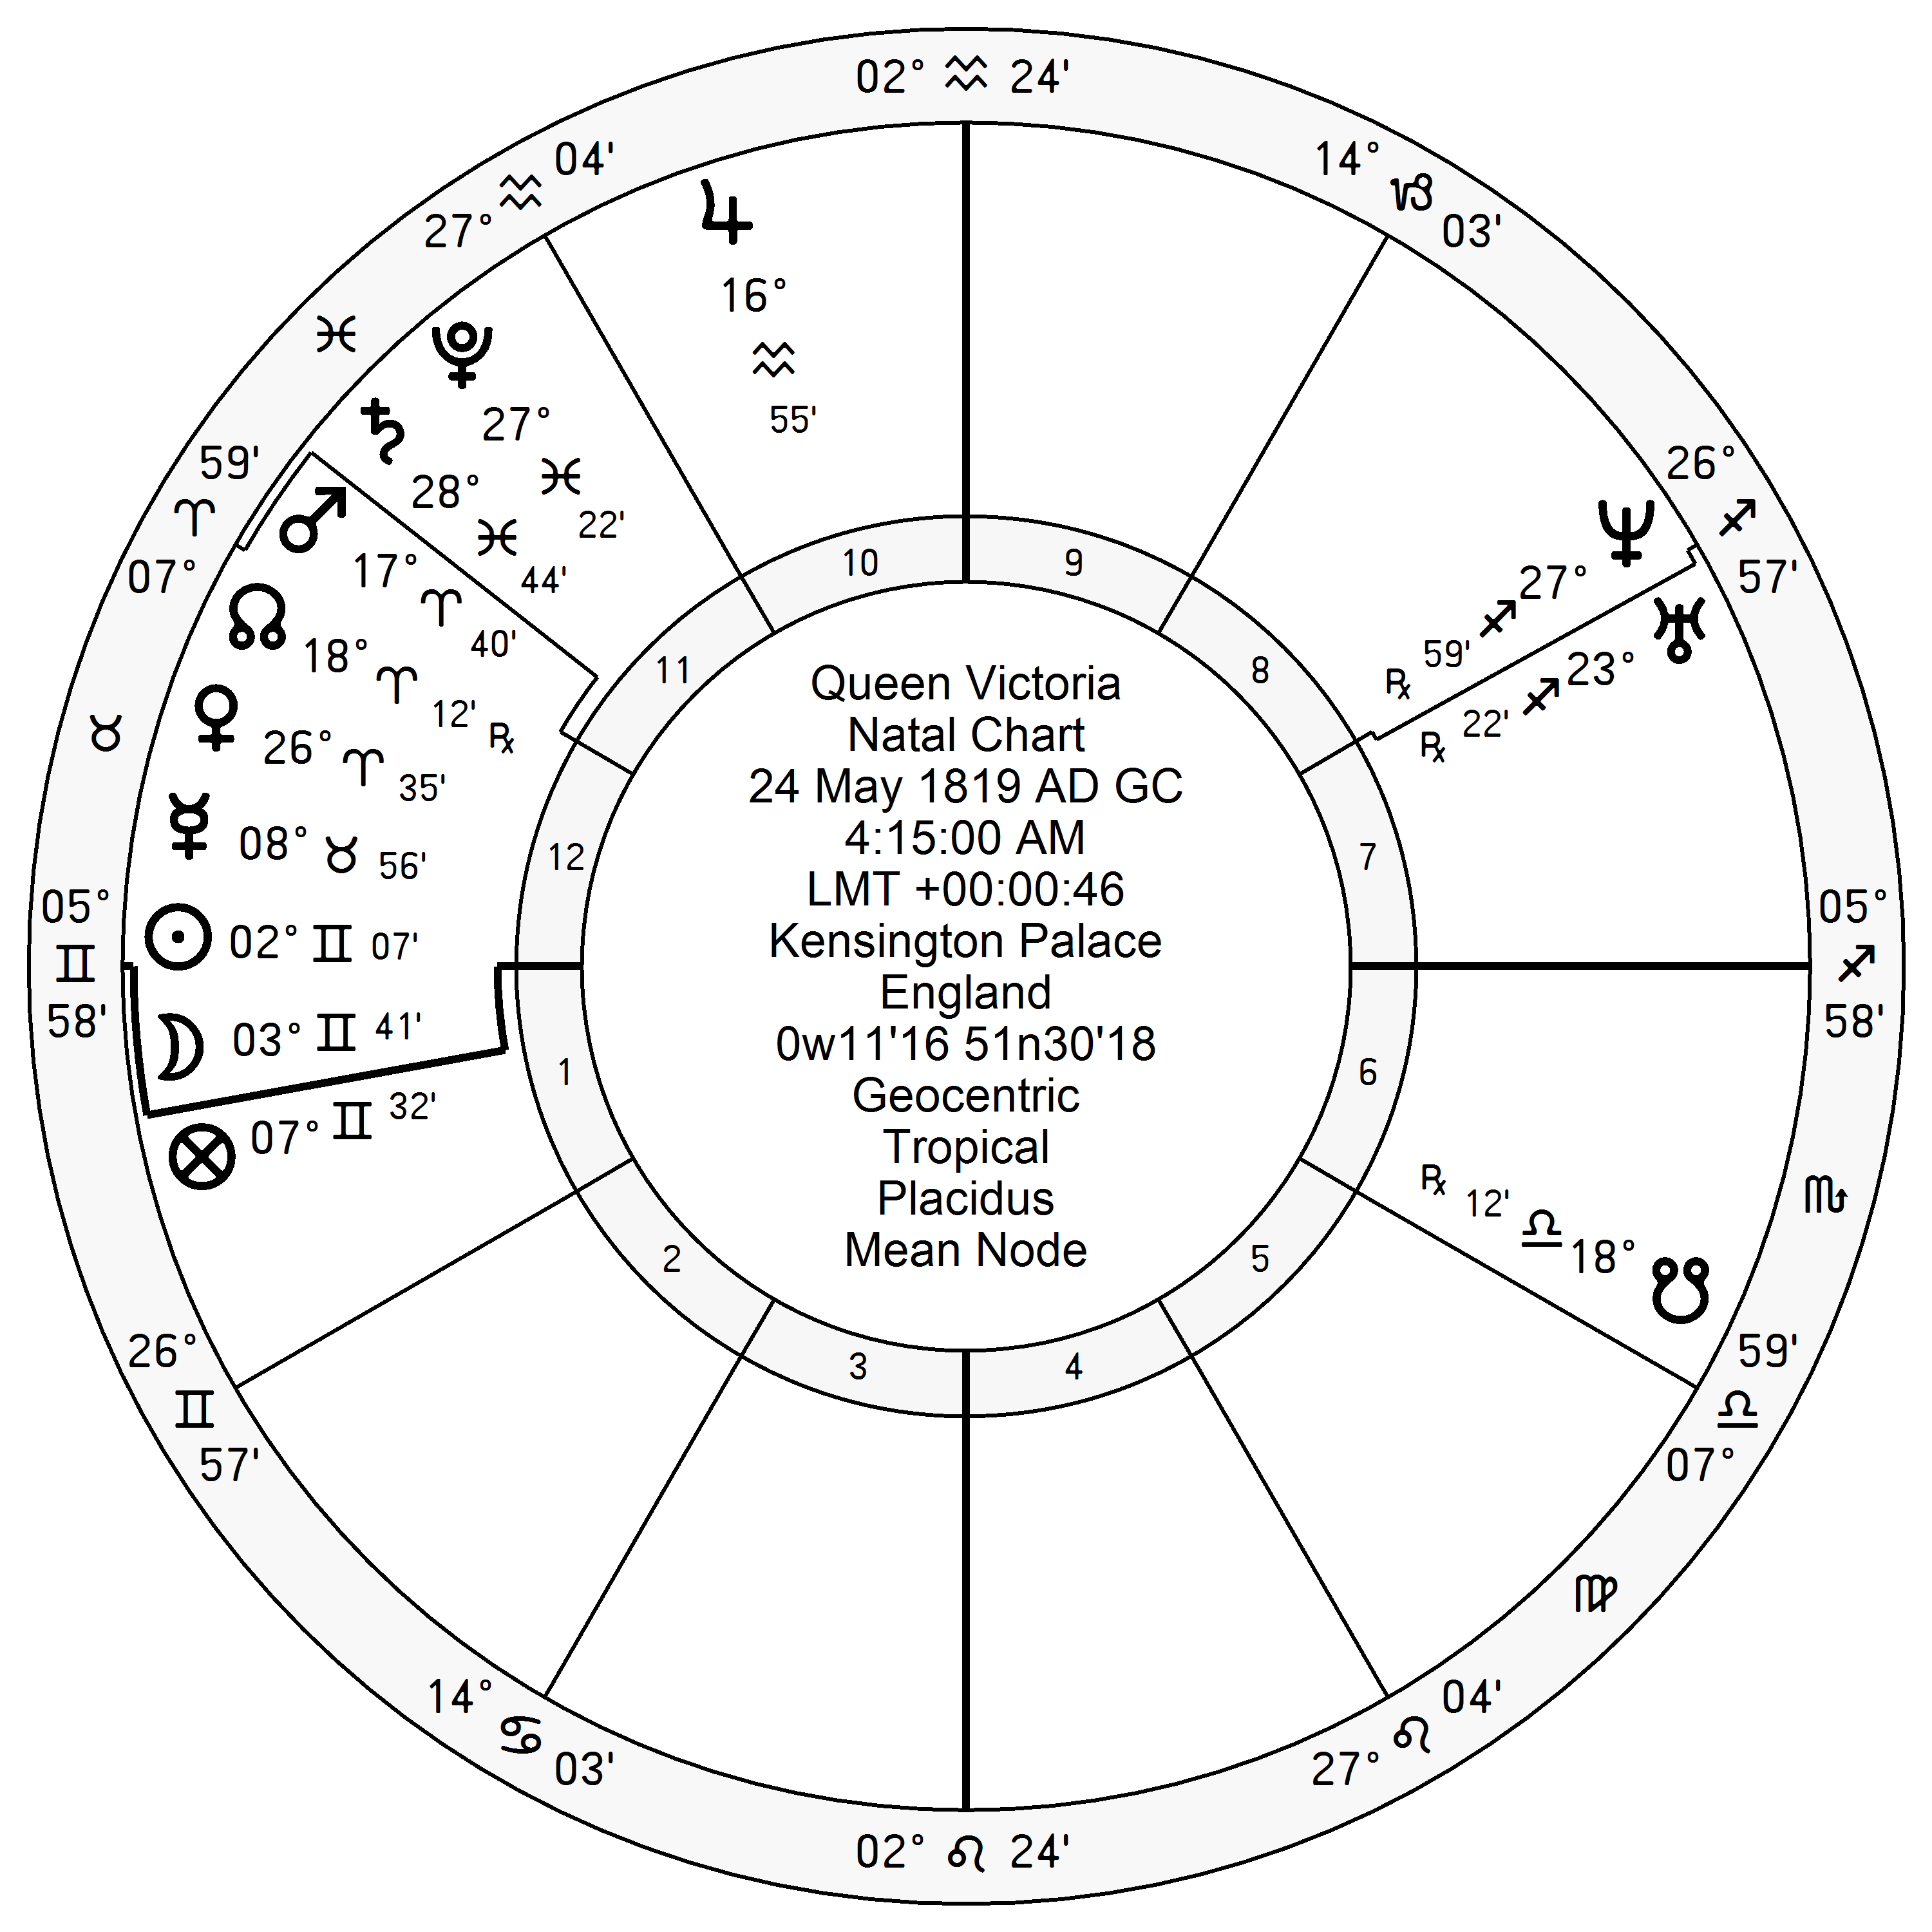
\includegraphics[width=0.7\textwidth]{charts/Victoria.png}
\caption{Chart 07: Queen Victoria}
\end{figure}

To know which planet ruled on June 20, 1837, the day she became Queen, we can take the day's Julian Day number (2392181)\footnotemark[1] and subtract the Julian Day number of her birth (2385579) to get 6,602 days since her birth then 6602 MOD 7 gives a remainder of 1 (6602/7 = 943. 6602-943*7=1) making the day ruler \Mercury, which is the ruler of her Ascendant. [At least, I think that's what Dorotheus' method boils down to.]

\footnotetext[1]{Julian Date calculator's are available on line; \href{https://core2.gsfc.nasa.gov/time/julian.html}{NASA} provides a good one.}

Once we've found the planet ruling the day we're investigating, he says to look for the sign the Moon is in and
\begin{quote}
\mn{1.60-62}\textsl{If the Moon is in that sign which the days reached and a malefic was in that sign in the nativity, then disease and evil will reach them [the natives]. Similarly if the place is bad [and] if a malefic aspects it at that time or this is the sign in which \Saturn\, or \Mars\, was in the base-nativity and this sign is the house of [one of] the malefics but benefics aspect it in transit, then his case will be middling. If this is reverse, then reverse it.}
\end{quote} 
\begin{quote}
\mn{1.60-64}\textsl{Look at the Moon which, of the benefics and malefics aspects it. If the planet which aspects the Moon is a benefic at the beginning of fifteen degrees [within its sign], then this day will be hard for the native, but on that night he will find rest and recovery in the morning.
}
\end{quote}

He appears to be saying we should judge the day according to the position of the day ruler and the relation of the transit Moon to the birth chart Moon. 